\section{Results of simulation}
\begin{frame}
  \frametitle{Simulation setup}
  \begin{itemize}
  \item[-] \alert{emulated} Kuka FRI Joint specific impedance control mode
    \begin{itemize}
    \item[] $\boldsymbol{\tau}_{cmd} = K_j(\vec{q}_{FRI} - \vec{q}_{msr}) + D(d_{j}) + \boldsymbol{\tau}_{FRI} + \vec{f}_{dynamics}(\vec{q}, \dot{\vec{q}}, \ddot{\vec{q}})$
    \end{itemize}
  \item[-] $K_j = 0$
  \item[-] $\vec{q}_{FRI} = \vec{q}_{msr}$
  \item[-] $d_{j} = 0$
  \item[-] $\vec{f}_{dynamics}$ supposed to be $\vec{G}$ evaluated using KDL library
    \footnote[frame]{The Kinematics and Dynamics Library (KDL) develops an application independent framework for modelling and computation of kinematic chains}
  \item[-] $\boldsymbol{\tau}_{FRI}$ used as commanded torque
  \end{itemize}
\end{frame}

\begin{frame}[shrink=15]
  \frametitle{Simulation setup (continued)}
  \begin{flalign*}
    &\boldsymbol{\tau}_{FRI} = C \dot{\vec{q}} + \cancel{\vec{G}} + B \vec{a}_{p2p}\\
    &\boldsymbol{\tau}_{FRI} = C \dot{\vec{q}} + \cancel{\vec{G}} +
    {}^{b}J^{T}_{S} ( B_A \vec{a}_{cmd} - B_A {}^{ws} \dot{J_{A,E}} \dot{\vec{q}}
    + {}^b\vec{w}_{S}) +  (I_7 - ({}^{b}J^{T}_{S}) ({}^{b} \bar{J}^{T}_{S})) \vec{\gamma}_{0}
  \end{flalign*}
  
  \begin{itemize}
  \item[-] controllers running @ $1$kHz
  \item[-] $G$ canceled because the gravity is compensated by the robot
  \item[-] $B$ given by KDL %{\color{dgreen}\cmark}
  \item[-] $C \dot{\vec{q}}$ given by KDL %{\color{dgreen}\cmark}
  \item[-] only $\vec{q}$ is available (as in the real scenario)
    \begin{itemize}
    \item[-] $\dot{\vec{q}}$ estimated using an exponential smoothing
      $\dot{\vec{q}}_k = (1 - \alpha) \dot{\vec{q}}_{k-1} + \alpha \frac{\vec{q}_k - \vec{q}_{k-1}}{t_s}$%{\color{orange}\cmark}
    \end{itemize}
    
  \item[-] Jacobians are evalutated using KDL library %{\color{dgreen}\cmark} 

  \item[-] $\vec{w}_F$ given by force/torque sensor sofware plugin
    \begin{itemize}
    \item[-] corrupted signal when the end-effector is mounted on the sensor $\longrightarrow$ massless tool%{\color{orange}\cmark}
    \end{itemize}
  \item[-] joints friction and contact friction neglected for ease of simulation %{\color{orange}\cmark}
  \item[-] generic end-effector instead of the hand for ease of simulation

  \end{itemize}
\end{frame}

\begin{frame}{Description of the simulated scenarios}
  The following scenarios were simulated in the Gazebo robot simulator
  \begin{columns}
    \begin{column}{0.5\textwidth}
      \begin{itemize}
        \item[-]contact phase
        \item[-]force regulation 
        \item[-]simultaneous force regulation and dragging
      \end{itemize}
    \end{column}
    \begin{column}{0.5\textwidth}
      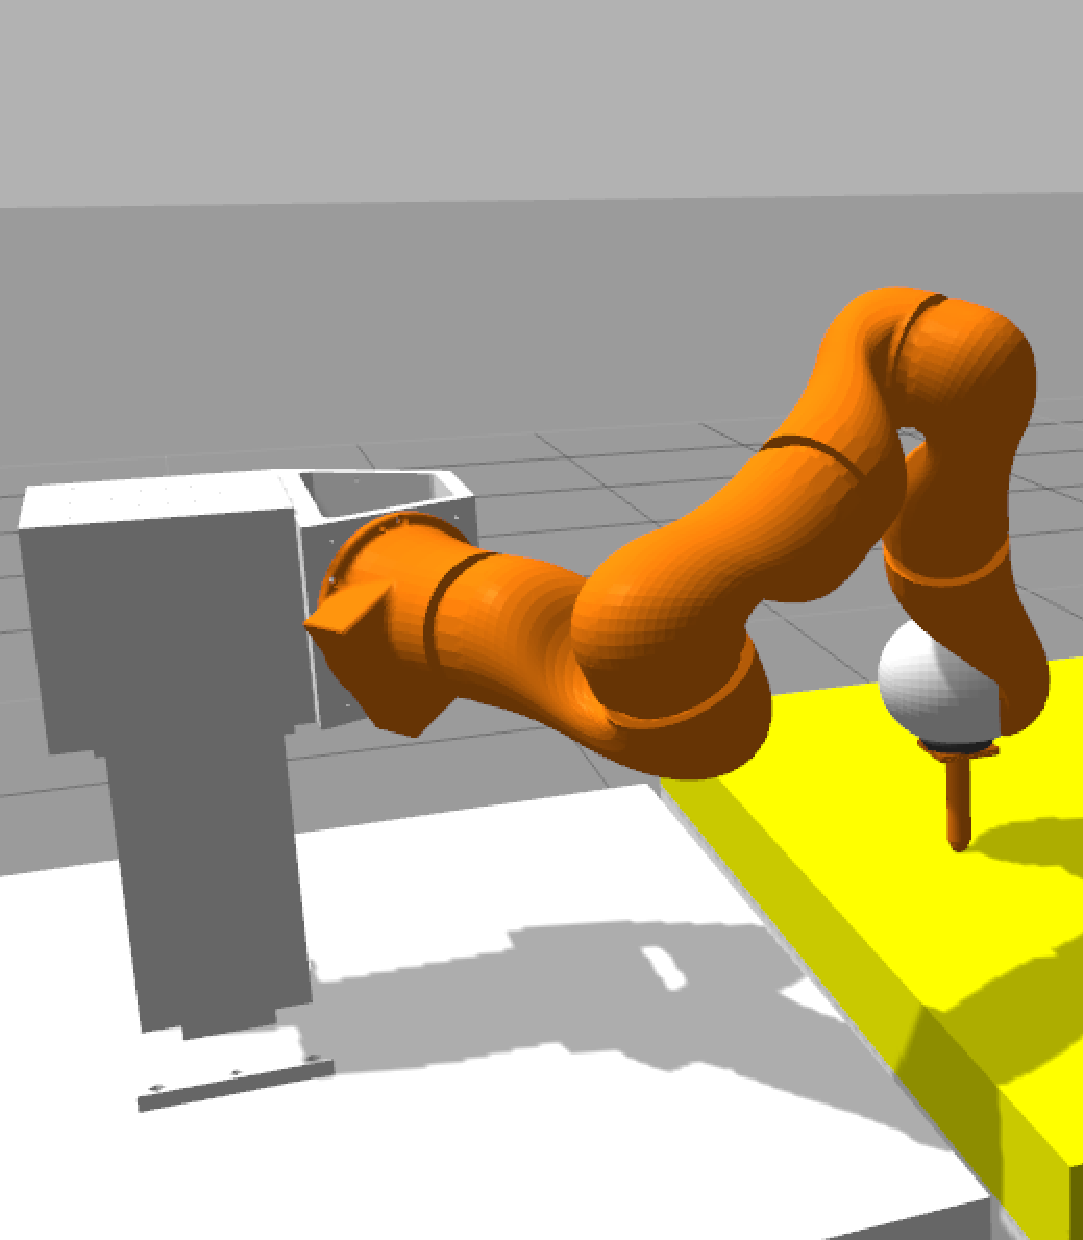
\includegraphics[width=\columnwidth]{task_picture}
    \end{column}
  \end{columns}
\end{frame}

\begin{frame}{Results - Force regulation}
  \begin{block}{Contact phase \hfill$K_f \in \{2,3\}, K_d = 25$}
    \vskip0.03in
    \begin{columns}
      \begin{column}{0.38\textwidth}
        %% simulation_press_err_y.pdf
        %% simulation_press_y.pdf
        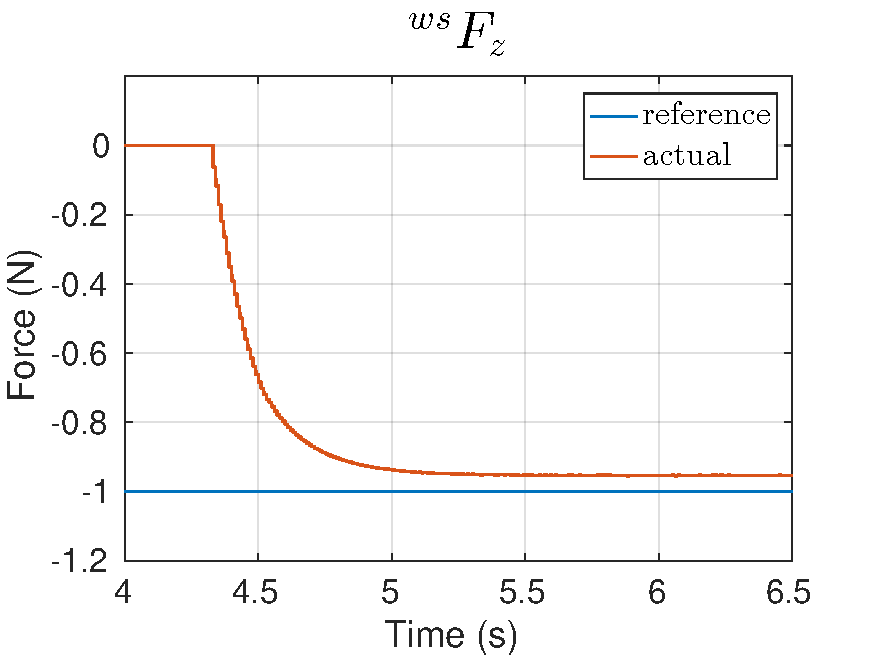
\includegraphics[width=\columnwidth]{simulation_contact1_z}
      \end{column}
      \begin{column}{0.38\textwidth}
        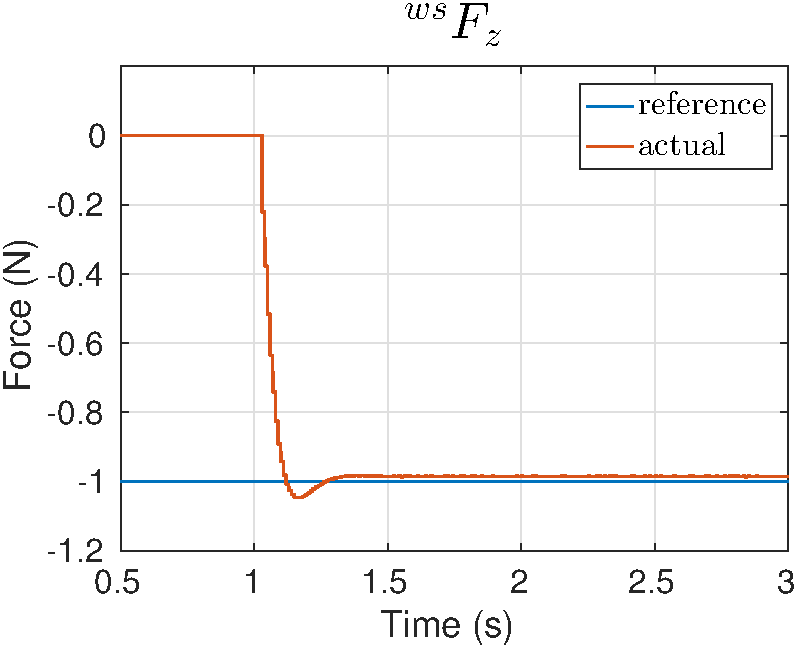
\includegraphics[width=\columnwidth]{simulation_contact2_z}
      \end{column}
    \end{columns}
  \end{block}
  \begin{block}{Force setpoint \hfill$K_f = 3, B_f = 45 $}
    \vskip0.03in
    \begin{columns}
      \begin{column}{0.38\textwidth}
        %% simulation_press_err_y.pdf
        %% simulation_press_y.pdf
        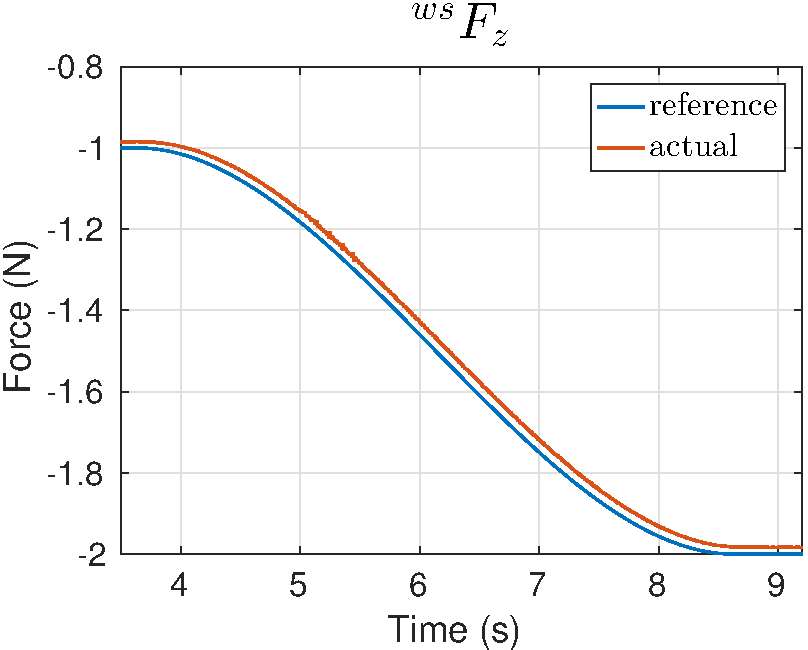
\includegraphics[width=\columnwidth]{simulation_press_z}
      \end{column}
      \begin{column}{0.38\textwidth}
        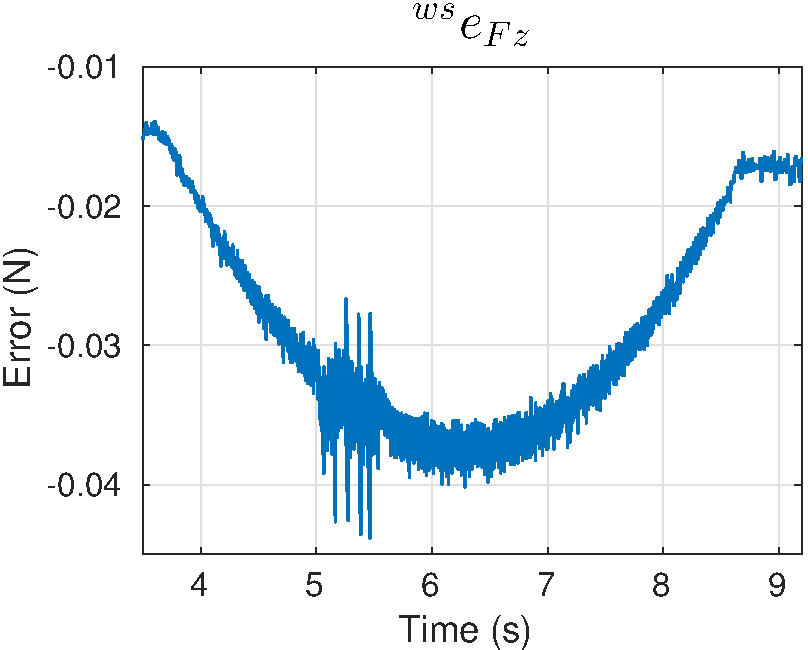
\includegraphics[width=\columnwidth]{simulation_press_err_z}
      \end{column}
    \end{columns}
  \end{block}
\end{frame}

\begin{frame}{Results - Dragging and Force regulation \hfill($K_f = 3, B_f = 45 $)}
  \vskip0.1in
  \begin{columns}
    \begin{column}{0.45\textwidth}
      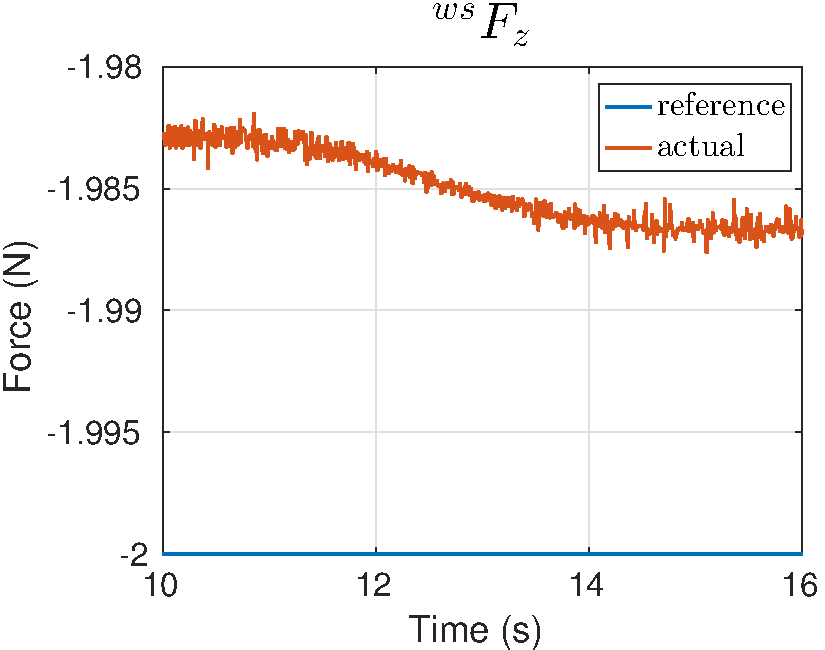
\includegraphics[width=\columnwidth]{simulation_move_z}\\
      \vskip0.1in
      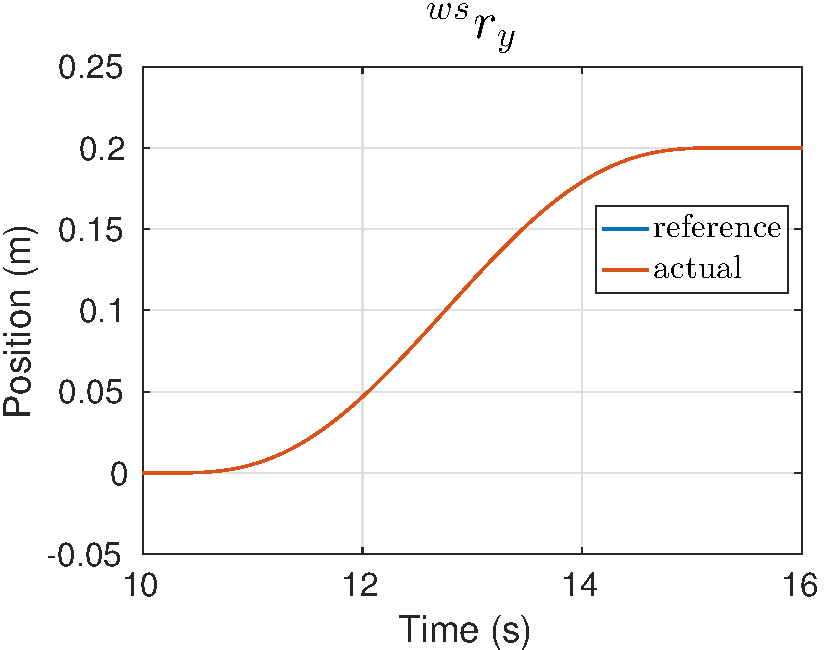
\includegraphics[width=\columnwidth]{simulation_move_y}
    \end{column}
    \begin{column}{0.45\textwidth}
      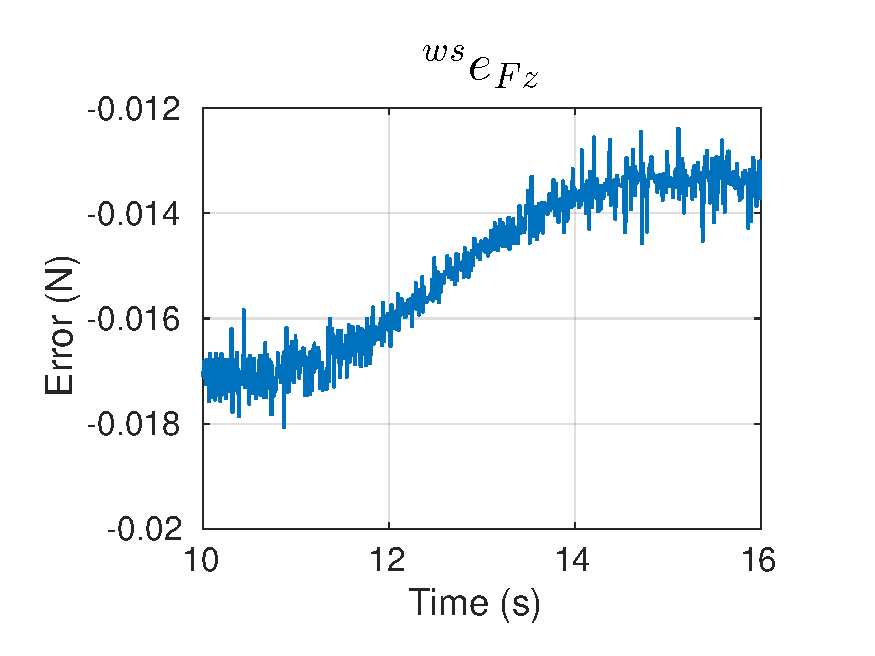
\includegraphics[width=\columnwidth]{simulation_move_err_z}\\
      \vskip0.1in
      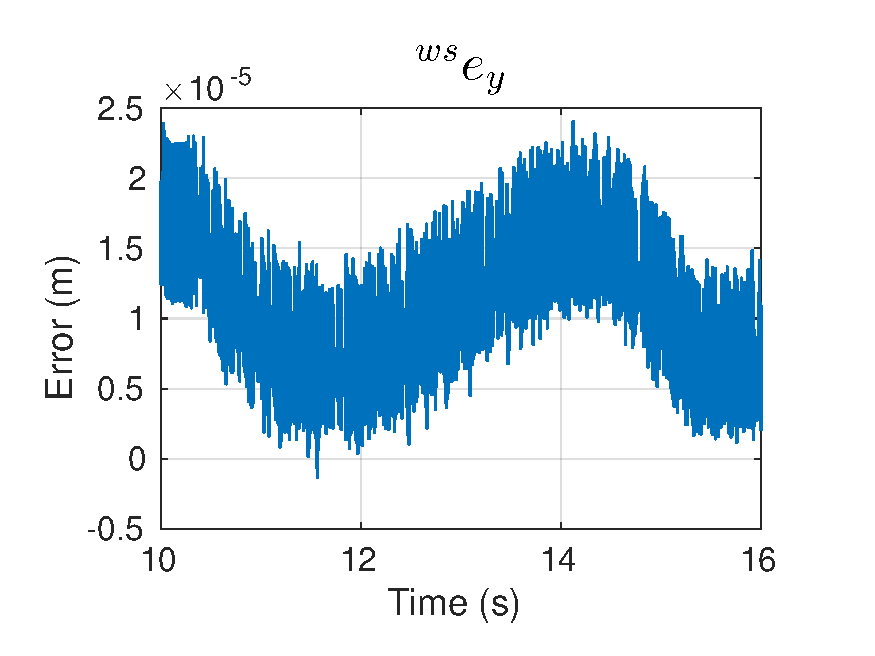
\includegraphics[width=\columnwidth]{simulation_move_err_y}
    \end{column}
  \end{columns}
\end{frame}
